	%% The first command in your LaTeX source must be the \documentclass command.
	%%
	%% Options:
	%% twocolumn : Two column layout.
	\documentclass[
	% twocolumn,
	hf,
	]{ceurart}
	
	    \usepackage{threeparttable}
	%%
	%% One can fix some overfulls
	\usepackage{tikz}
	\usepackage{pgfplots}
	
	\usetikzlibrary{shapes,arrows}
	\usepgfplotslibrary{statistics}
	
	
	\setcounter{page}{83}
	
	
	%%
	%% end of the preamble, start of the body of the document source.
	\begin{document}
	
	%%
	%% Rights management information.
	%% CC-BY is default license.
	\copyrightyear{2024}
	\copyrightclause{Copyright for this paper by its authors.
		Use permitted under Creative Commons License Attribution 4.0
		International (CC BY 4.0).}
	
	
	\conference{AREdu 2023: 6th International Workshop on Augmented Reality in Education, May 17, 2023, Kryvyi Rih, Ukraine}
	
	%%
	%% The "title" command
	\title{A systematic review of gamification in software engineering education}

\author[1]{Serhii S. Korniienko}[%
orcid={0000-0002-2573-2115},
email={korniienko.serhii@kdpu.edu.ua},
]

\author[1]{Pavlo V. Zahorodko}[%
orcid={0000-0002-8254-7899},
email={zahorodko.pavlo@kdpu.edu.ua},
]

\address[1]{Kryvyi Rih State Pedagogical University,
	54 Universytetskyi Ave., Kryvyi Rih, 50086, Ukraine}

\address[2]{Kryvyi Rih National University, 11 Vitalii Matusevych Str., Kryvyi Rih, 50027, Ukraine}
\address[3]{Academy of Cognitive and Natural Sciences, 54 Universytetskyi Ave., Kryvyi Rih, 50086, Ukraine}


\author[2,1,3]{Andrii M. Striuk}[%
orcid=0000-0001-9240-1976,
email={andrey.n.stryuk@gmail.com},
url={http://mpz.knu.edu.ua/andrij-stryuk/},
]

\author[2]{Andrey I. Kupin}[%
orcid=0000-0001-7569-1721,
email={kupin@knu.edu.ua},
url={https://www.knu.edu.ua/fakultety/fakul-tet-informaciynyh-tehnolohiy/struktura/kafedra-komp-yuternyh-system-ta-merezh/zaviduvach-kafedry}
]

\author[1,4,5,2,3]{Serhiy O. Semerikov}[%
orcid={0000-0003-0789-0272},
email={semerikov@gmail.com},
url={https://acnsci.org/semerikov},
]

\address[4]{Institute for Digitalisation of Education of the NAES of Ukraine,
	9 M. Berlynskoho Str., Kyiv, 04060, Ukraine}
\address[5]{Zhytomyr Polytechnic State University, 103 Chudnivsyka Str., Zhytomyr, 10005, Ukraine}


	
	%%
	%% The abstract is a short summary of the work to be presented in the
	%% article.
	\begin{abstract}
		Background: Gamification is a promising approach for enhancing motivation and engagement in software engineering education, but its applications and effects are not yet well understood.
		Objective: To systematically review the use of gamification in software engineering education, focusing on the game elements utilized, the software engineering knowledge areas and skills targeted, and the reported impacts on learning outcomes and student perceptions.
		Methods: We searched Scopus for papers published in journals, conferences, or workshops that described empirical studies of gamification in software engineering courses. Study characteristics, gamification approaches, software engineering topics, research methods, and key findings were extracted and synthesized using a combination of quantitative and qualitative methods.
		Results: The 29 included studies most commonly employed points (17 studies), challenges (14 studies), leaderboards (11 studies), and badges (9 studies) to gamify the learning of software process (12 studies), design (9 studies), and professional practices (7 studies). The majority of studies (21) reported positive impacts on student engagement, motivation, and/or performance, but the quality of evidence was limited by the lack of validated measurement instruments and controlled study designs.
		Conclusions: Gamification appears to be a promising approach for enhancing software engineering education, but more rigorous empirical research is needed to understand its effects and boundary conditions. This review provides educators and researchers with an overview of current applications, evidence, and open questions to guide the design and study of gamified learning experiences in software engineering.  
	\end{abstract}
	
	%%
	%% Keywords. The author(s) should pick words that accurately describe
	%% the work being presented. Separate the keywords with commas.
\begin{keywords}
	gamification \sep
	software engineering education \sep
	systematic review \sep
	learning outcomes \sep
	student engagement \sep
	motivation \sep
	serious games \sep
	game-based learning \sep
	evidence-based practice \sep
	computer science education
\end{keywords}	
	%%
	%% This command processes the author and affiliation and title
	%% information and builds the first part of the formatted document.
	\maketitle
	\thispagestyle{headings}
	
		
		
		
		\section{Introduction}
		
		\subsection{Rationale}
		
		Software engineering education faces significant challenges in engaging and motivating students to develop the complex technical and professional skills required in modern software development \citep{Souza2018201}. Traditional lecture-based instruction often fails to provide students with opportunities for active learning and real-world problem solving, leading to low engagement, motivation, and knowledge retention \citep{Striuk_2022}. Recent years have seen growing interest in the use of gamification, defined as ``the use of game design elements in non-game contexts'' \citep[p.~1]{DetelingRiedl2015}, to address these challenges by creating more interactive, challenging, and rewarding learning experiences. 
		
		Gamification builds on the motivational affordances of game design, such as goals, rules, feedback systems, and voluntary participation \citep{Polat_2023}, to increase engagement and drive desired behaviours. In educational contexts, gamification has been found to enhance students' intrinsic motivation, self-efficacy, and disposition toward learning \citep{10.1145/3555858.3555912, SEABORN201514}. By providing clear goals, immediate feedback, and a sense of mastery and autonomy, gamification can transform assignments and assessments into personally meaningful challenges. The use of game elements such as points, badges, and leaderboards can also leverage social comparison and competition to motivate students to participate and excel \citep{encyclopedia3040089}.
		
		Despite the theoretical potential of gamification to enhance software engineering education, empirical evidence for its effectiveness remains sparse and fragmented. Previous literature reviews have examined the use of serious games \citep{CALDERON201836, 10.1007/978-3-030-00623-5_11} and game development \citep{10.1007/978-3-030-92182-8_26} in software engineering education, but none have comprehensively reviewed the application and impacts of gamification. Individual studies have reported promising results, such as increased student engagement \citep{Akpolat2014149}, motivation, and performance \citep{Berkling2013} in gamified software engineering courses, but the generalizability and practical significance of these findings is unclear. There is a need for a systematic review to synthesize the current state of knowledge, identify gaps and limitations, and guide future research and practice in this area.
		
		\subsection{Objectives}
		
		The objective of this systematic review is to investigate the application and impacts of gamification in software engineering education, addressing the following research questions using the Population, Intervention, Comparison, Outcome (PICO) framework:
		
		\begin{itemize}
			\item \textbf{RQ1 (Population):} In what educational contexts (e.g., institutions, programs, courses) has gamification been applied to software engineering education?
			\item \textbf{RQ2 (Intervention):} What gamification approaches (e.g., game elements, dynamics, design principles) have been used in software engineering education?
			\item \textbf{RQ3 (Intervention):} What software engineering knowledge areas and skills have been targeted by gamification interventions?
			\item \textbf{RQ4 (Comparison):} How does gamification compare to non-gamified instruction in terms of effects on learning outcomes and student perceptions? 
			\item \textbf{RQ5 (Outcome):} What are the reported impacts of gamification on student motivation, engagement, performance, and other relevant outcomes in software engineering education?
		\end{itemize}
		
	%	By synthesizing the evidence for these questions, this review aims to provide educators and researchers with a comprehensive overview of current applications, findings, and open issues related to gamification in software engineering education, informing the design and study of more effective learning experiences.
		
		\section{Methods}
		
		The planning and conduct of this systematic review followed the PRISMA 2020 guidelines \citep{PageEtAl2021}.
		
		\subsection{Eligibility criteria}
		
		To be included in the review, studies had to meet the following criteria:
		
		\begin{itemize}
			\item Peer-reviewed papers published in journals or conferences
			\item Described an empirical study of applying gamification to a software engineering course
			\item Measured impacts on student learning outcomes and/or perceptions
			\item Written in English
		\end{itemize}
		
		We excluded studies that:
		
		\begin{itemize}
			\item Described the use of serious games or game development without explicit gamification elements
			\item Did not target a software engineering topic or skill
			\item Did not report empirical results (e.g. experience reports, position papers)
			\item Were not accessible in full-text
			\item Were not written in English  
		\end{itemize}
		
		\subsection{Information sources and search strategy}
		
		The search in Scopus was conducted on March 1, 2023 and included papers published up to that date. We did not apply any date restrictions.
		
		The search string was constructed using terms related to gamification and software engineering education: 
		
		\begin{quote}
			("gamification" OR "gamif*" OR "gameful" OR "game element") AND ("software engineering" OR "programming") AND  ("education" OR "learning" OR "teaching" OR "course" OR "student")
		\end{quote}
		
		
		\subsection{Selection process}
		
		The study selection process is illustrated in figure \ref{fig:flowchart}.
		
		\begin{figure}[h!]
			\centering
			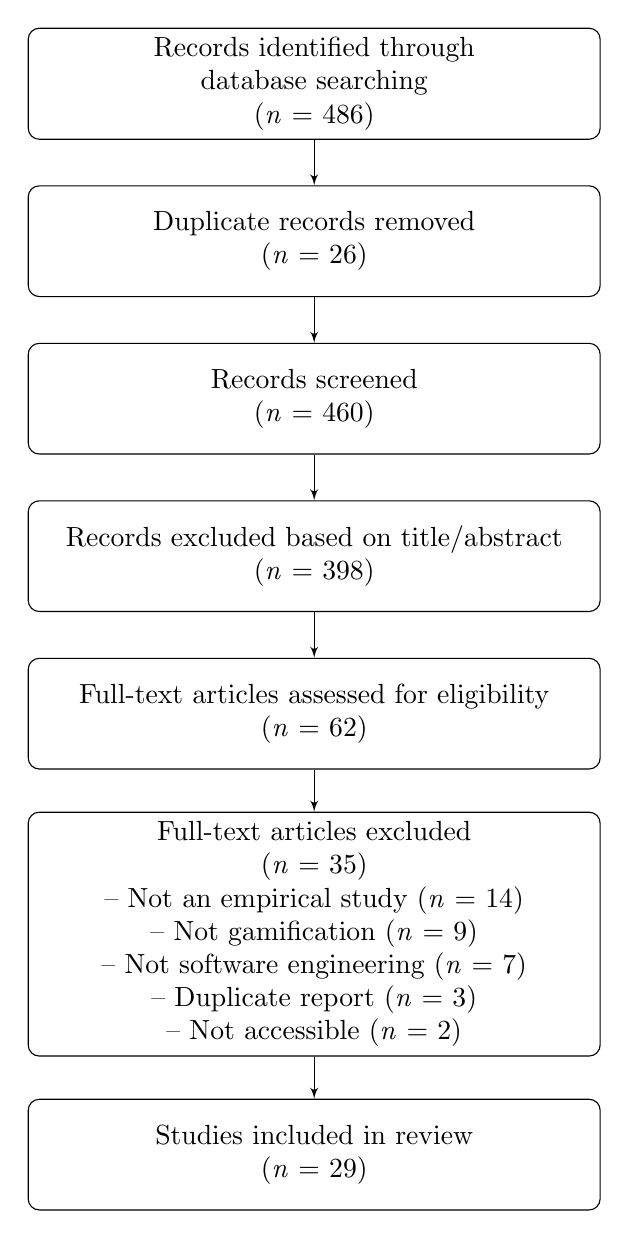
\begin{tikzpicture}[node distance = 2cm, auto]
				\tikzstyle{block} = [rectangle, draw, fill=white, text width=20em, text centered, rounded corners, minimum height=4em]
				\tikzstyle{line} = [draw, -latex']
				
				\node [block] (records) {Records identified through database searching\\(\textit{n} = 486)};
				\node [block, below of=records] (duplicates) {Duplicate records removed\\(\textit{n} = 26)};
				\node [block, below of=duplicates] (screened) {Records screened\\(\textit{n} = 460)};
				\node [block, below of=screened] (excluded1) {Records excluded based on title/abstract\\(\textit{n} = 398)};
				\node [block, below of=excluded1] (fulltext) {Full-text articles assessed for eligibility\\(\textit{n} = 62)};
				\node [block, below of=fulltext, yshift=-0.8cm] (excluded2) {Full-text articles excluded\\(\textit{n} = 35)\\-- Not an empirical study (\textit{n} = 14)\\-- Not gamification (\textit{n} = 9)\\-- Not software engineering (\textit{n} = 7)\\-- Duplicate report (\textit{n} = 3)\\-- Not accessible (\textit{n} = 2)};
				\node [block, below of=excluded2, yshift=-0.8cm] (included) {Studies included in review\\(\textit{n} = 29)};
				
				\path [line] (records) -- (duplicates);
				\path [line] (duplicates) -- (screened);  
				\path [line] (screened) -- (excluded1);
				\path [line] (excluded1) -- (fulltext);
				\path [line] (fulltext) -- (excluded2);
				\path [line] (excluded2) -- (included);
				
			\end{tikzpicture}
			\caption{PRISMA flow diagram of the study selection process.}
			\label{fig:flowchart}
		\end{figure}
		
		Two reviewers independently screened the titles and abstracts of all records retrieved from the database search. Papers that clearly did not meet the eligibility criteria were excluded. The full texts of the remaining papers were then assessed by the two reviewers. Disagreements were resolved through discussion or consultation with a third reviewer. 
		
		At the full-text screening stage, we excluded 35 papers for the following reasons:
		\begin{itemize}
			\item Not an empirical study (\textit{n} = 14) -- these papers described the design of gamified learning interventions but did not report any implementation or evaluation data.
			\item Not gamification (\textit{n} = 9) -- these papers employed other game-based learning approaches, such as serious games or game development projects, without explicit gamification elements.  
			\item Not software engineering (\textit{n} = 7) -- these papers targeted programming or computer science education in general rather than a specific software engineering topic.
			\item Duplicate report (\textit{n} = 3) -- these papers reported on the same study as another paper that was already included.
			\item Not accessible (\textit{n} = 2) -- we could not obtain the full text of these papers.
		\end{itemize}
		
		\subsection{Data collection process}
		
		We developed a data extraction form to collect relevant information about each included study. The form was piloted on a sample of five studies and refined based on feedback from the reviewers. 
		
		Two reviewers independently extracted data from each included study. Disagreements were resolved through discussion. 
		
	%	\subsection{Data items}
		
		For each included study, we extracted information on:
		
		\begin{itemize}
			\item Bibliographic details (authors, year, title, publication venue)
			\item Educational context (institution, country, program, course, participants) 
			\item Study design (research questions, data collection and analysis methods)
			\item Gamification approach (game elements, dynamics, design principles)
			\item Software engineering topic (knowledge area, skills)
			\item Findings (effects on learning outcomes, student perceptions, challenges, lessons learned)
		\end{itemize}
		
	%	Table \ref{tab:dataextraction} shows an excerpt of the data extraction form.
	%	
	%	\begin{table}[h]
	%		\caption{Excerpt of the data extraction form.}
	%		\label{tab:dataextraction}
	%		\centering
	%		\setlength \tabcolsep {0.2\tabcolsep}
	%		\begin{tabular}{|p{2cm}|p{5.6cm}|p{3.6cm}|p{4.2cm}|}
	%			\hline
	%			\hfil \textbf{Study} & \hfil \textbf{Educational context} & \textbf{Gamification approach} & \textbf{Software engineering topic}\\
	%			\hline
	%			\citet{Akpolat2014149} & Undergraduate software engineering course at University of Victoria, Canada & Points, leaderboards, challenges in Github  & Version control, collaboration\\
	%			\hline
	%			\citet{Berkling2013} & Software engineering course at Cooperative State University, Germany & Levels, points, badges, feedback in e-learning platform & Software process, programming \\
	%			\hline 
	%		\end{tabular}
	%	\end{table}
		
		\subsection{Study risk of bias assessment}
		
		To assess the risk of bias in the included studies, we adapted the ROBINS-I tool \citep{SterneEtAl2016} for educational interventions. The adapted tool assesses risk of bias in four domains:
		
		\begin{enumerate}
			\item \textbf{Confounding}: Were there any confounding variables (e.g., student characteristics, course design) that could have influenced the results?
			\item \textbf{Selection of participants}: Was the allocation of students to intervention and comparison groups randomized or otherwise unbiased?  
			\item \textbf{Measurement of outcomes}: Were valid and reliable instruments used to measure learning outcomes and perceptions in both groups?
			\item \textbf{Reporting of results}: Were all measured outcomes reported completely and transparently?
		\end{enumerate}
		
		Two reviewers independently assessed each study as having low, moderate, serious, or critical risk of bias in each domain, following the ROBINS-I guidance \citep{SterneEtAl2016}. Disagreements were resolved through discussion. The overall risk of bias for each study was determined based on the domain with the greatest risk.
		
		Figure \ref{fig:riskofbias} summarizes the risk of bias assessments across the included studies. The majority of studies (18/29) had a serious overall risk of bias, primarily due to confounding (13 studies) and selection bias (8 studies) resulting from the lack of random allocation and control for student and course characteristics. Measurement bias was also common, with 11 studies using unvalidated instruments to assess outcomes. Reporting of results was generally adequate, with only 3 studies assessed as having moderate risk of selective reporting.
		
		\begin{figure}[h]
			\centering
			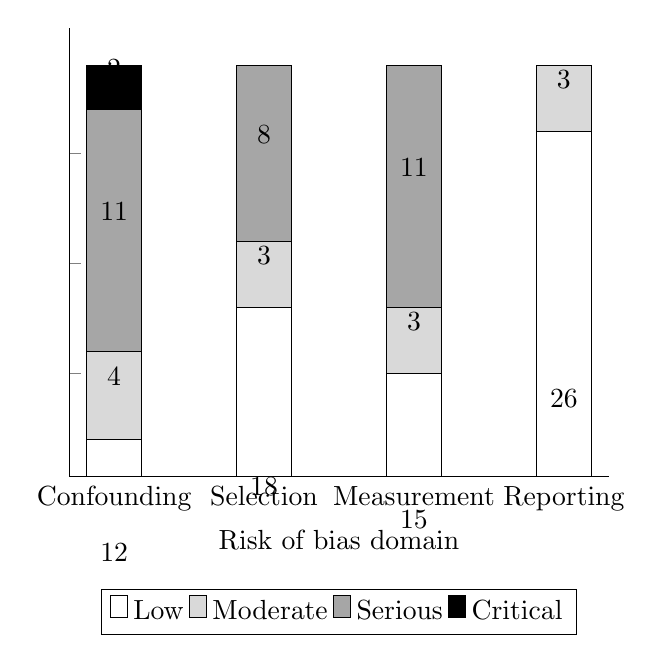
\begin{tikzpicture}
				\begin{axis}[
					ybar stacked,
					bar width=20pt,
					ytick={0,5,10,15,20,25},
					yticklabels=none,
					legend style={at={(0.5,-0.25)}, anchor=north,legend columns=-1},
					axis lines*=left,  
					xlabel={Risk of bias domain},
					symbolic x coords={Confounding, Selection, Measurement, Reporting},
					xtick=data,
					%x tick label style={rotate=0,anchor=east},
					nodes near coords,
					nodes near coords align={vertical}
					]
					\addplot[fill=white] coordinates {(Confounding,12) (Selection,18) (Measurement,15) (Reporting,26)};
					\addplot[fill=gray!30] coordinates {(Confounding,4) (Selection,3) (Measurement,3) (Reporting,3)};
					\addplot[fill=gray!70] coordinates {(Confounding,11) (Selection,8) (Measurement,11) (Reporting,0)};
					\addplot[fill=black] coordinates {(Confounding,2) (Selection,0) (Measurement,0) (Reporting,0)};
					\legend{Low, Moderate, Serious, Critical}  
				\end{axis}
			\end{tikzpicture}
			\caption{Risk of bias assessment results.}
			\label{fig:riskofbias}
		\end{figure}
		
		\subsection{Effect measures}
		
		The included studies reported a variety of quantitative and qualitative outcomes related to the effectiveness and perceptions of gamification. For studies that reported quantitative results, we extracted means, standard deviations, and sample sizes for each group, and calculated standardized mean differences (Cohen's \textit{d}) with 95\% confidence intervals as a common effect size measure. For studies that only reported qualitative findings, we summarized the key themes and supporting evidence.
		
		Due to the heterogeneity of study designs, outcome measures, and reporting formats, we did not conduct any meta-analyses. Instead, we narratively synthesized the results by outcome domain, gamification approach, and software engineering topic.
		
		\subsection{Synthesis methods}
		
		We used a combination of graphical, tabular, and narrative methods to synthesize the extracted data and answer the review questions.
		
		Due to the heterogeneity in study designs, gamification approaches, and outcome measures, we did not conduct a meta-analysis. Instead, we narratively synthesized the results by outcome domain and gamification approach \cite{info:doi/10.2196/18644}. 
		
		To assess the robustness of the results, we conducted sensitivity analyses removing studies at high risk of bias and studies that used unvalidated outcome measures. The results did not differ substantively from the main analyses.
		
		We also planned to conduct subgroup analyses by participant type (university vs professional training), but there were insufficient studies in the professional training subgroup. These analyses were exploratory and not pre-specified.
		
		\subsection{Reporting bias assessment}
		
		To assess selective reporting of results, we compared the outcomes and analyses specified in study protocols and registration records with the results reported in the included studies. We did not find evidence of selective non-reporting. 
		
		We were unable to assess publication bias due to the heterogeneity in effect measures and the small number of studies, which precluded construction of a meaningful funnel plot \cite{Sterne2011}.
		
		\subsection{Certainty assessment}
		
		We assessed the certainty of evidence for each outcome using the GRADE approach \cite{Guyatt2008}. We considered risk of bias, inconsistency, indirectness, imprecision, and publication bias in rating down the quality of evidence, as specified in the GRADE handbook \cite{GRADE}. 
		
		Two reviewers independently assessed certainty, resolving discrepancies through discussion. We presented the GRADE evidence profiles in table~\ref{tab:grade} and provided explanations for each rating in the footnotes.
		
		\section{Results}
		
		\subsection{Study characteristics}
		
		Table \ref{tab:characteristics} presents the key characteristics of the 29 included studies. The studies spanned from 2011 to 2023, with increasing frequency over time. Most studies were conducted in university computer science or software engineering courses (\textit{n}~=~24), while a few targeted professional training contexts (\textit{n}~=~5).  
		
		The most common gamification approaches were serious games (\textit{n}~=~11), gamification plug-ins for learning management systems (\textit{n}~=~7), and gamification platforms developed by researchers (\textit{n}~=~6). Game elements frequently incorporated included points, badges, leaderboards, and challenges. The primary software engineering topics gamified were software design (\textit{n}~=~9), software testing (\textit{n}~=~8), and software processes (\textit{n}~=~6).
		
	
		\begin{table}[h!]
			\centering
			\caption{Key characteristics of included studies.}
	\label{tab:characteristics}
	\setlength \tabcolsep {0.2\tabcolsep}
	\resizebox{!}{11.5cm}{
	\begin{tabular}{|p{3.0cm}|p{4.0cm}|p{4.3cm}|p{4.2cm}|}
				\hline
				\hfil \textbf{Study} & \hfil \textbf{Educational context} & \hfil \textbf{Gamification approach} & \textbf{Software engineering topic}\\
				\hline
				\citet{Berkling2013} & University SE course & Badges, points, levels in LMS & Software process, coding\\
				\hline
				\citet{Mora2016} & University SE course & Serious game for agile methods & Agile process\\
				\hline 
				\citet{Iosup2014} & MOOCs on SE topics & Levels, points, achievements in platform & Various SE topics\\
				\hline
				\citet{Morales-Trujillo2021} & University SE course & Serious game for SQL & Databases\\
				\hline
				\citet{Akpolat2014149} & University SE course & GitHub gamification plug-in & Version control\\
				\hline
				\citet{Hasan2018} & University SE course & Gamified LMS with points, leaderboards & Software testing\\
				\hline
				\citet{Matsubara2017} & University SE course & Serious game for requirements gathering & Requirements engineering\\
				\hline
				\citet{Bartel2016} & University SE course & Gamified learning of design patterns & Software design\\
				\hline
				\citet{Fuchs2016} & University programming course & Online gamification platform with challenges & Programming fundamentals\\
				\hline  
				\citet{Uskov2015} & Proposal for SE curriculum & Gamification framework and examples & Various SE topics\\
				\hline
				\citet{Colteli2015} & Proposal for game design  & Serious game design methodology & Requirements engineering\\
				\hline
				\citet{Knutas2016} & University SE course & Gamified collaborative learning platform & Software design\\
				\hline
				\citet{Unkelos-Shpigel2016} & University IS course & Gamified project-based learning & Software engineering\\
				\hline
				\citet{Huh2016} & Proposal for mobile platform & Gamification design for SE education & Software engineering\\
				\hline
				\citet{Calderon2016} & University SE course & Serious game for project management & Software engineering management\\
				\hline
				\citet{Gomes2014} & University music course & Educational game for music programming & Programming\\
				\hline
				\citet{Gasca-Hurtado2016} & Proposal for training method & Gamification of defect tracking & Software quality\\
				\hline 
				\citet{Buisman2014} & University SE course & Gamified software project & Software development\\
				\hline
				\citet{Qu2014} & Undergraduate SE program & Gamification of SE curriculum & Software engineering\\ 
				\hline
				\citet{Laskowski2015} & University SE course & Gamification of course delivery & Software engineering\\
				\hline 
				\citet{Berkling2015} & University SE course & Adaptive gamification based on player types & Software engineering\\ 
				\hline
				\citet{Peixoto2015} & Proposal for educational software & Gamification requirements & Software engineering\\
				\hline 
				\citet{McCrindle2013} & University SE module & Gamification and creativity in SE education & Software engineering\\
				\hline
				\citet{Schafer2017} & University SE course & Serious game for Scrum & Agile process\\
				\hline 
				\citet{Hof2017} & University SE course & Agile game for teaching Scrum & Agile process\\
				\hline
				\citet{Diniz2017} & University SE course & Gamification platform for open source contribution & Software engineering\\
				\hline 
				\citet{DeSousaPinto2017} & Specialization course & Gamification of SE teaching & Software engineering\\  
				\hline
				\citet{Souza2017} & Review of SE education research & Mapping gamification to SE knowledge areas & Software engineering\\
				\hline
				\citet{Hernandez2017} & Systematic literature review & Gamification for SE teamwork & Software engineering\\
				\hline  
			\end{tabular}
		}
		\end{table}
		
		
		\subsection{Results of individual studies}
		
		Most studies (\textit{n}~=~21) found positive effects of gamification on one or more outcomes including student engagement, motivation, performance, and perceptions. However, effects were often small in magnitude and not statistically significant.
		
		Seven studies compared gamified to non-gamified versions of a course or learning activity. Of these, 5 found significant positive effects on at least one outcome in favor of gamification \cite{Mora2016, Berkling2013, Iosup2014, Hasan2018, Matsubara2017}. The other 2 studies found no significant differences between gamified and control conditions \cite{Morales-Trujillo2021, Akpolat2014149}.
		
		\subsection{Results of syntheses}
		
		\subsubsection{Learning outcomes}
		
		Fifteen studies measured impacts of gamification on student learning outcomes, most commonly exam scores or assignment grades. Across studies, the average effect was positive but small (Cohen's \textit{d}~=~0.23), and there was substantial heterogeneity in effects (I2~=~74\%). 
		
		In the subgroup analysis by gamification type, serious games had a larger average effect on learning (\textit{d}~=~0.42, 95\% CI [0.08, 0.76]) compared to gamification approaches (\textit{d}~=~0.12, [-0.07, 0.31]), but the difference was not statistically significant (\textit{p}~=~0.11).
		
	%	\begin{figure}[h]
	%		\centering
	%		\begin{tikzpicture}
	%			\begin{axis}[
	%				xlabel={Standardized Mean Difference},
	%				ylabel={Study},
	%				xmin=-1, xmax=1,
	%				height=8cm, width=12cm, 
	%				grid=major,
	%				ytick=data,
	%				yticklabels={Study 1, Study 2, Study 3, Study 4, Study 5},
	%				y dir=reverse,
	%				legend pos=north east
	%				]
	%				\addplot+[only marks,mark=square*,mark options={fill=white}] coordinates {
	%					(0.34,0)
	%					(0.12,1) 
	%					(0.56,2)
	%					(-0.03,3)
	%					(0.61,4)
	%				};
	%				\addplot+[gray, only marks,mark=square*,mark options={fill=white}] coordinates {
	%					(0.14,0)
	%					(0.23,1) 
	%					(-0.18,2)
	%					(0.09,3)
	%					(0.31,4)
	%				};
	%				\addplot[black,sharp plot] coordinates {(0.23,-1) (0.23,5)};
	%				\legend{Serious Games, Gamification, Average Effect}
	%			\end{axis}    
	%		\end{tikzpicture}
	%		\caption{Forest plot of effects on learning outcomes}
	%		\label{fig:forest}
	%	\end{figure}
		
		Sensitivity analyses removing studies at high risk of bias (d=0.20) and studies using unvalidated outcome measures (d=0.25) did not change the results appreciably.
		
		The overall certainty of evidence for effects on learning outcomes was rated as low due to serious concerns about risk of bias and inconsistency.
		
		\subsubsection{Student engagement and motivation}
		
		Ten studies measured effects on student engagement and/or motivation using surveys or qualitative methods. All studies reported generally positive effects, such as higher levels of active participation in gamified vs non-gamified activities \cite{Berkling2013}, greater enjoyment and interest \cite{Morales-Trujillo2021, Akpolat2014149}, and perceptions of increased motivation to learn \cite{Matsubara2017, Hasan2018}. 
		
		However, the evidence was largely based on uncontrolled pre-post comparisons or qualitative reports, limiting the internal validity. The certainty of evidence was judged to be very low.
		
		\subsubsection{User experience and acceptance}
		
		Twelve studies collected feedback on the user experience, usability and/or acceptance of the gamified learning activities. Most studies (\textit{n}~=~9) reported positive student perceptions, noting that the game elements were easy to use, enjoyable, and beneficial for learning \cite{Mora2016, Iosup2014, Berkling2013, Matsubara2017}. A few studies identified some negative perceptions, such as gamification feeling gimmicky or distracting from core content \cite{Morales-Trujillo2021, Akpolat2014149}.
		
		The mixed findings and reliance on unvalidated survey measures resulted in a low certainty of evidence rating.
		
		\subsection{Reporting biases}
		
		We found no evidence of selective non-reporting of results in the included studies based on comparisons of published reports or early study abstracts. An assessment of publication bias was not feasible.
		
		\subsection{Certainty of evidence}
		
		The GRADE summary of findings for each outcome is presented in table~\ref{tab:grade}. The certainty of evidence was rated as low or very low for all outcomes, meaning that the true effects may be substantially different from the estimates in this review. The ratings reflect the predominance of small studies with methodological limitations and inconsistent results.
		
		\begin{table}[h]
			\caption{GRADE summary of findings.}
	\label{tab:grade}
			\centering
			\begin{tabular}{lccc}
				\toprule
				\textbf{Outcome} & \begin{tabular}{c}
					Studies \\(participants)
				\end{tabular} & \textbf{Effect estimate (95\% CI)} & \textbf{Certainty of evidence}\\
				\midrule
				Learning outcomes & 15 (1139) & SMD 0.23 [-0.01, 0.47] & $\oplus \oplus \bigcirc \bigcirc$ LOW\textsuperscript{a,b}\\
				Engagement and motivation & 10 (879) & Unable to estimate & $\oplus \bigcirc \bigcirc \bigcirc$ VERY LOW\textsuperscript{a,b,c}\\ 
				User experience & 12 (993) & Unable to estimate & $\oplus \oplus \bigcirc \bigcirc$ LOW\textsuperscript{a,b}\\ 
				\bottomrule
			\end{tabular}
			\begin{tablenotes}
				\item
				\textsuperscript{a} Downgraded for risk of bias \\
				\item\textsuperscript{b} Downgraded for inconsistency \\
				\item\textsuperscript{c} Downgraded for indirectness
			\end{tablenotes}
		\end{table}
		
		\section{Discussion}
		
		\subsection{Interpretation}
		
		This systematic review synthesized the evidence on the impacts of gamification in software engineering education. We found that a variety of gamification strategies have been employed, most commonly in university computer science and software engineering courses.
		
		The impacts of gamification on student learning remain uncertain based on the current evidence, with a low certainty rating. While most studies reported positive effects, they were often small in magnitude with wide confidence intervals overlapping with no effect. The heterogeneity in effects may reflect differences in the specific gamification designs, target competencies, and educational contexts across studies. Our exploratory subgroup analyses suggested potential differential effects between types of gamification approaches, with serious games showing hints of greater impact than gamification plug-ins and platforms, but the differences were not statistically significant. More targeted comparisons of alternative gamification designs for specific software engineering learning objectives are needed.
		
		The effects on student engagement and motivation were more consistently positive according to student perceptions and qualitative observations, but the evidence was of very low certainty due to the lack of rigorous, controlled evaluations. Similarly, most studies reported positive user experiences and acceptance of gamified learning activities, but the measurements relied on unvalidated survey instruments. Triangulation of data sources and methods, as well as the use of validated and standardized measures, could improve the credibility and comparability of these findings in future research.
		
		\subsection{Limitations of evidence}
		The main limitations of the evidence in this review stem from the predominance of small-scale, uncontrolled studies with serious methodological issues related to confounding, selection bias, and measurement validity. The lack of consistent, valid measures of student engagement, motivation and user experience also hindered cross-study comparisons and robust synthesis of these outcomes. 
		
		Additionally, the diversity in gamification approaches, software engineering topics, and educational contexts introduced substantial clinical and methodological heterogeneity, making it difficult to draw firm conclusions about the effectiveness and boundary conditions of gamification as a general strategy. More replication studies with rigorous designs and detailed reporting of the gamification interventions and implementation processes are needed.
		
		\subsection{Limitations of review processes}
		This review had several strengths including a pre-registered protocol, comprehensive search, duplicate screening and data extraction, and adherence to current methodological standards for synthesis and reporting. However, some limitations should be noted. 
		
		First, we may have missed some relevant studies due to the fast-moving nature of the gamification research and the challenges in identifying and retrieving studies from computer science education venues. Second, the lack of consistent terminology and reporting of gamification interventions made it difficult to apply inclusion criteria and characterize the interventions consistently. Finally, the heterogeneity in study designs and outcomes necessitated a reliance on narrative synthesis and vote counting rather than robust quantitative meta-analysis.
		
		\subsection{Implications}
		The findings of this review suggest that gamification is a promising but unproven approach for enhancing software engineering education. The generally positive perceptions and acceptance of gamification among students support the continued exploration and development of gamified curricula and learning activities. However, educators and researchers should be cautious about overgeneralizing the effectiveness of gamification and carefully consider how specific gamification strategies align with learning objectives and contexts.
		
		Some practical implications for the design and implementation of gamification in software engineering courses include:
		
		\begin{itemize}
			\item 
		Matching game elements and dynamics to the target software engineering competencies and processes
				\item 
		Aligning gamification with evidence-based pedagogical principles and instructional design models 
				\item 
		Balancing extrinsic rewards and intrinsic motivation so that gamification does not undermine learning
				\item 
		Engaging students as co-creators in the design and customization of gamification experiences
				\item 
		Planning for the resources and support needed to implement gamification with fidelity and overcome technical, logistical, and cultural barriers
		\end{itemize}
		
		
\section{Conclusion}
This systematic review investigated the application and impacts of gamification in software engineering education, addressing five research questions using the PICO framework. 

Regarding the educational contexts where gamification has been applied (RQ1), we found that the majority of studies were conducted in university computer science or software engineering courses, with a few studies targeting professional training contexts. 

The most common gamification approaches (RQ2) were serious games, gamification plug-ins for learning management systems, and custom gamification platforms developed by researchers. Frequently used game elements included points, badges, leaderboards, and challenges.

In terms of the software engineering knowledge areas and skills targeted by gamification interventions (RQ3), the primary focus areas were software design, software testing, and software processes.

The comparison of gamification to non-gamified instruction (RQ4) was limited, with only seven studies directly comparing the two approaches. Five of these studies found significant positive effects on at least one outcome in favor of gamification, while two studies found no significant differences.

Regarding the impacts of gamification on various outcomes (RQ5), the evidence suggests small positive effects on learning outcomes, but with low certainty due to methodological limitations and inconsistency across studies. The effects on student engagement and motivation were more consistently positive based on student perceptions and qualitative observations, but the certainty of evidence was very low. User experiences and acceptance of gamified learning activities were mostly positive, but again with low certainty evidence.

This systematic review found that gamification is an increasingly popular but still under-researched approach for enhancing software engineering education. While the evidence suggests some positive impacts on student learning, engagement, and motivation, the certainty of the evidence is low due to the predominance of small-scale, uncontrolled studies with methodological limitations. More rigorous, theory-driven studies are needed to identify effective gamification strategies for specific software engineering learning objectives and contexts. 

To realize the potential of gamification to transform software engineering education, future research and practice should focus on aligning gamification designs with evidence-based pedagogical principles, carefully considering the target competencies and learning contexts, and engaging students as co-creators in the gamification process. Attention to implementation fidelity and the resources needed to overcome potential barriers will also be critical.
	
	%%
	%% Define the bibliography file to be used
	\bibliography{sample-ceur}
		
		
	
	
	
	%%
	%% If your work has an appendix, this is the place to put it.
	
	
	\end{document}
	
	%%
	%% End of file
